\documentclass[10pt]{article}
\usepackage{acl}
\usepackage{fontspec}
\usepackage{polyglossia}
\usepackage{latexsym}
\usepackage{microtype}
\usepackage{booktabs}
\usepackage{array}
\usepackage{graphicx}
\setdefaultlanguage{russian}
\setotherlanguage{english}
\defaultfontfeatures{Ligatures=TeX}
\setmainfont{Times New Roman}[Ligatures=TeX]
\setsansfont{Arial}[Ligatures=TeX]
\setmonofont{Courier New}[Ligatures=TeX]
\newfontfamily\cyrillicfont{Times New Roman}[Ligatures=TeX]
\newfontfamily\cyrillicfontsf{Arial}[Ligatures=TeX]
\newfontfamily\cyrillicfonttt{Courier New}[Ligatures=TeX]
\setlength{\textfloatsep}{6pt plus 2pt minus 2pt}
\setlength{\floatsep}{4pt plus 2pt minus 2pt}
\setlength{\intextsep}{6pt plus 2pt minus 2pt}
\makeatletter
\def\@listi{\leftmargin\leftmargini
            \topsep 2pt plus 1pt minus 1pt
            \parsep 0pt
            \itemsep 1pt}
\let\@listI\@listi
\@listi
\makeatother

\title{ДЗ0: критерии оценки веб-поисковиков}
\author{Георгий Мамарин}

\begin{document}
\maketitle

\section{Коротко}
Смущенный форматом сдачи и непривычностью работы в такой структуре, в этом отчете я предлагаю набор критериев для оценки веб-поисковиков и показываю, как по ним можно сравнить Google, Yandex, ChatGPT и Gemini. Основная идея состоит в том, что для классического поиска и для LLM-инструментов нужны частично различающиеся критерии, а итоговая оценка должна учитывать тип запроса и исходную потребность пользователя.

\section{Постановка задачи}
Если оценивать поисковик только через общую «релевантность», мы потеряем различия между задачами. Навигационный запрос вроде \texttt{вшэ факультет компьютерных наук} требует быстро найти один конкретный сайт, а запрос на сравнение или объяснение требует скорее хорошего покрытия темы и удобного ответа. На мой взгляд, оценка поисковика должна быть завязана на тип информационной потребности пользователя.

Традиционный подход к поиску качественно изменился из-за глубины проникновения LLM-инструментов. В классическом поиске пользователь чаще получает список ссылок, из которых он делает вываод самостоятельно, прокликивая их одну за другой. А в ChatGPT или Gemini он часто получает уже готовый ответ, который может проверить через подобранные источники, если LLM подкрепит ими свою генерацию. Из-за этого сравнивать все системы одной и той же метрикой становится мало разумным: для части задач важнее ранжирование документов, а для другой --- качество синтезированного ответа.

\section{Критерии оценки}
Мне кажется, критерии удобнее описывать не как длинный список, а как несколько более общих измерений.

Первое измерение --- это \textbf{качество поиска}. Для традиционных поисковиков его разумно измерять стандартными метриками:
\begin{itemize}
\item \texttt{Success@1} или \texttt{MRR} для навигационных запросов;
\item \texttt{NDCG@10} для информационных запросов;
\item \texttt{Recall@k} или покрытием аспектов для более исследовательских сценариев.
\end{itemize}
Они хорошо отражают ситуацию, когда система возвращает ранжированный список документов.

Второе измерение --- \textbf{качество самого ответа}. Для LLM-инструментов одного качества ранжирования мало. Здесь нужно отдельно смотреть на:
\begin{itemize}
\item \textbf{корректность ответа};
\item \textbf{наличие опоры на источники};
\item \textbf{галлюцинации}, то есть случаи, когда система уверенно выдает неподтвержденные утверждения.
\end{itemize}
Иными словами, хороший ответ должен быть не только удобным, но и проверяемым.

Третье измерение --- \textbf{стоимость достижения результата для пользователя}. Даже если система в конце концов приводит к верному ответу, важно, сколько шагов для этого нужно: придется ли переформулировать запрос, переходить по нескольким ссылкам или давать дополнительные вводные.

Четвертое измерение --- \textbf{устойчивость к реальным запросам}. Здесь я бы выделил:
\begin{itemize}
\item \textbf{задержку} --- слишком медленный ответ ухудшает пользовательский опыт;
\item \textbf{устойчивость к нечетким и неоднозначным запросам};
\item \textbf{локальную и языковую адаптацию} --- насколько система хорошо работает с русским языком, локальным контекстом и смешанными запросами.
\end{itemize}

Пятое измерение --- \textbf{доверие к системе}. Сюда входят:
\begin{itemize}
\item видимость ссылок и источников;
\item понятность происхождения ответа;
\item отсутствие навязчивости;
\item \textbf{приватность} --- часть пользователей будет предпочитать менее навязчивую систему, соглашаясь на возможное падение качества.
\end{itemize}

Чтобы сделать итоговую оценку зависимой от сценария, предлагаю ввести три профиля задач:
\begin{itemize}
\item \textbf{навигационный веб-поиск} --- важнее всего качество поиска, скорость и низкая стоимость достижения результата;
\item \textbf{исследовательский / сравнительный поиск} --- важнее качество синтеза, проверяемость и возможность быстро собрать ответ из нескольких источников;
\item \textbf{русскоязычный локальный поиск} --- важнее языковая адаптация, локальный контекст и устойчивость к реальным пользовательским формулировкам.
\end{itemize}

Для этих профилей можно использовать разные веса по укрупненным измерениям:
\begin{table}[t]
\centering
\footnotesize
\setlength{\tabcolsep}{2.2pt}
\renewcommand{\arraystretch}{1.08}
\resizebox{\columnwidth}{!}{%
\begin{tabular}{>{\raggedright\arraybackslash}p{0.39\columnwidth}ccccc}
\toprule
\textbf{Профиль} & \textbf{Поиск} & \textbf{Ответ} & \shortstack[c]{\textbf{Стоимость}\\ \textbf{результата}} & \shortstack[c]{\textbf{Устойчи-}\\ \textbf{вость}} & \textbf{Доверие} \\
\midrule
Навигационный веб-поиск & 40\% & 5\% & 25\% & 20\% & 10\% \\
Исследовательский поиск & 10\% & 35\% & 20\% & 15\% & 20\% \\
Русскоязычный локальный поиск & 25\% & 10\% & 15\% & 35\% & 15\% \\
\bottomrule
\end{tabular}
}
\caption{Веса укрупненных измерений для разных профилей задач.}
\label{tab:weights}
\end{table}

\section{Набор сценариев}
Чтобы сравнение не было слишком узким, я бы включил в набор запросов шесть сценариев: навигационный (\texttt{вшэ факультет компьютерных наук}), информационный (\texttt{что такое BM25}), исследовательский (\texttt{сравнение BM25 и dense retrieval}), неоднозначный (\texttt{питон}), локальный (\texttt{кофейня рядом со мной}) и мультиязычный (\texttt{lemmatization для русского языка}). Такой набор покрывает не только «поиск факта», но и реальные случаи, где пользователю нужны уточнение запроса, локальная информация или сравнение нескольких источников.

Этот набор также учитывает различия между пользователями. Более опытным пользователям важнее качество источников и полнота покрытия темы. Массовым пользователям важнее скорость ответа и понятность интерфейса. Пользователям, которые заботятся о приватности, важно, насколько навязчиво система собирает данные и показывает рекламу.

\section{Краткое сравнение систем}
Таблица~\ref{tab:compare} показывает упрощенное качественное сравнение по шкале от 1 до 5. Это не полноценный эксперимент, а скорее способ показать, как выбранные критерии разделяют сильные и слабые стороны разных систем.

\begin{table}[t]
\centering
\footnotesize
\setlength{\tabcolsep}{2.8pt}
\renewcommand{\arraystretch}{1.08}
\resizebox{\columnwidth}{!}{%
\begin{tabular}{>{\raggedright\arraybackslash}p{0.42\columnwidth}cccc}
\toprule
\textbf{Критерий} & \textbf{Google} & \textbf{Yandex} & \textbf{ChatGPT} & \textbf{Gemini} \\
\midrule
Качество поиска & 5.0 & 5.0 & 2.0 & 3.0 \\
Качество ответа & 2.5 & 2.0 & 4.5 & 4.0 \\
Стоимость результата & 4.0 & 4.0 & 5.0 & 4.0 \\
Устойчивость & 4.0 & 5.0 & 4.0 & 3.5 \\
Доверие & 2.0 & 2.0 & 2.0 & 2.0 \\
\bottomrule
\end{tabular}
}
\caption{Базовые оценки по пяти укрупненным измерениям.}
\label{tab:compare}
\end{table}

Из такого сравнения видно две основные вещи. Во-первых, \textbf{традиционные поисковики остаются сильнее в поиске по вебу как таковому}. Google особенно хорош, когда нужно быстро найти каноническую страницу, свежие материалы или общемировые результаты. Яндекс особенно естественно выглядит в задачах с русскоязычными запросами, локальным контекстом и поиском по привычным российским сервисам.

Во-вторых, \textbf{LLM-системы сильнее там, где нужен синтез информации и снижение пользовательских усилий}. ChatGPT и Gemini удобнее для суммаризации, сравнения и последовательного уточнения вопроса. Но именно для них особенно важно проверять наличие источников: удобный и гладкий ответ без подтверждения не должен автоматически считаться хорошим результатом.

Если применить к этим оценкам веса из разных профилей задач, получится, что лидеры действительно меняются в зависимости от сценария: в навигационном и локальном русскоязычном профиле сильнее выглядят Google и Yandex, а в исследовательском профиле вперед выходят ChatGPT и Gemini.

\begin{figure}[t]
\centering
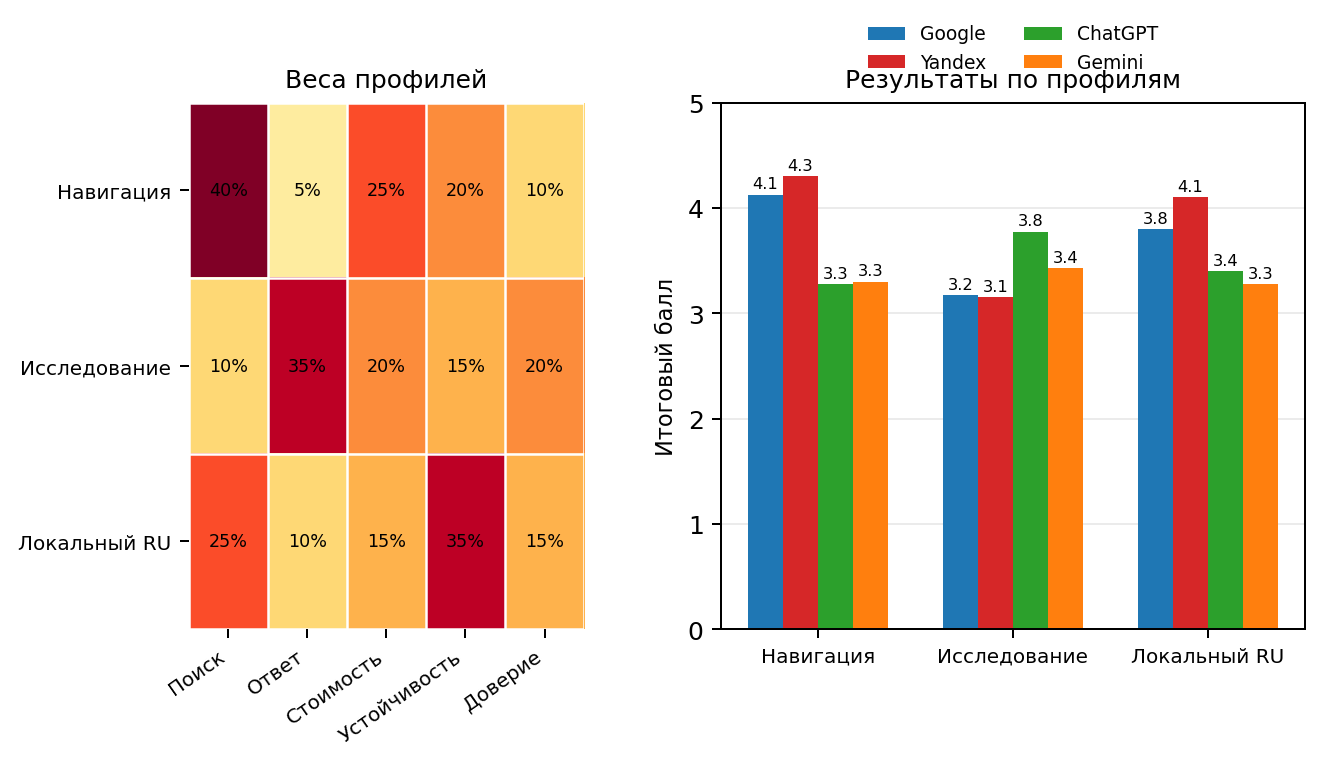
\includegraphics[width=0.92\columnwidth]{profile_scores.png}
\caption{Слева веса профилей задач, справа итоговые баллы систем при этих весах.}
\label{fig:profiles}
\end{figure}

\section{Заключение}
Таким образом, «лучший поисковик» нельзя определить одной общей метрикой. Корректнее оценивать системы по набору критериев, который зависит от сценария использования. Для классических поисковиков важнее релевантность, полнота, свежесть и задержка. Для LLM-инструментов к этому добавляются качество ответа, наличие источников и отсутствие галлюцинаций.

Практически это означает, что лучше подбирать не один универсальный сервис, а набор инструментов под россыпь задач.

\end{document}
